\documentclass{article}

\pagestyle{myheadings}

\usepackage{graphicx}
\usepackage{amsmath}
\usepackage{cite}
\usepackage{tikz}
\usepackage{verbatim}
\usepackage[active,tightpage]{preview}
\usepackage{fancyheadings}
\usepackage{graphicx}
\usepackage{lastpage}
\usepackage{hyperref}
\usepackage[symbol]{footmisc}

\pagestyle{fancy}

\fancyhead[C]{Team 53506}
\fancyhead[R]{Page \thepage\ of \pageref{LastPage}}
\fancyfoot{}

\title{Safer Migration Strategies For Refugee Populations}
\author{Team 53506}

\begin{document}

\pagenumbering{gobble}

\maketitle
\tableofcontents
\newpage

\pagenumbering{arabic}

\section{Introduction}

Humanitarian organizations are currently faced with a critical challenge; larger numbers of refugees are migrating than have been seen since the Second World War\cite{simpson}. This historical crisis lead to the formation of the UNHCR\footnote{United Nations High Commissioner for Refugees} in 1950\cite{historyUNHCR}. Since then, the organization has continually aided refugees, stateless and internally displaced peoples. With its historical reputation, the UNHCR has a primary imperative to find solutions to the current crisis. This paper considers mathematical models which aid the UNHCR in identifying important policies in guiding refugee migration.

We begin by splitting the modelling process into two separate modelling problems:
%
\begin{itemize}
    \item {\bf What are optimal migration pattern of refugee populations?}
    \item {\bf How do migration patterns influence exogenous factors during the immigration procedure?}
\end{itemize}
%
Moving refugees is modelled as a quadratic optimization. Simple arguments on the nature of the movement lead to well defined constraints. We attempt to find a solution which minimizes the `risk' of refugees, as derived later on in the paper. Based on this optimal movement, we construct a stochastic simulation model, which implements the planned routes\footnote{Due to time constraints, this part of the project was not implemented.}. Simulations of political opinion, based on the theories of opinion dynamics, lead us to consider the public's reaction to the procedure over time. Exogenous events may lie unconsidered in the original model, which may be seen during the simulation phase. Based on this data, the UN may take an informed decision on the crucial problem of refugee management.

\section{Background}

The 1951 refugee convention defines a refugee as

\begin{quote}
    ``owing to a well-founded fear of being persecuted for reasons of race, religion, nationality, membership of a particular social group or political opinion, is outside the country of his nationality, and is unable to, or owing to such fear, is unwilling to avail himself of the protection of that country'' \cite{1951convention}
\end{quote}
%
To contrast, a migrant is any emmigrating person without refugee status. In our discussion, we do not distinguish between migrants and refugees; Difficulties arise when distinguishing migrants and refugees in data, since refugees often lack official status.

\begin{figure}[h]
\begin{center}
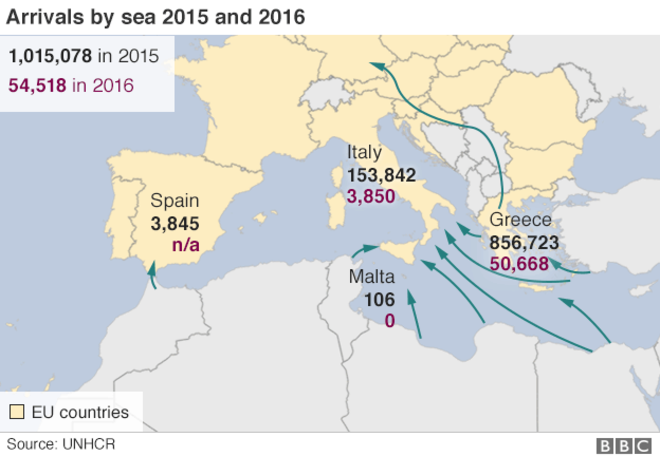
\includegraphics[scale=0.5]{travelmap}
\caption{Immigrants travel multiple routes -- beginning at the middle east, and travelling through the West, East, and Central Mediterranean, the West Balkans, the Eastern Borders, and from Albania to Greece. \cite{BBCgraphics}}
\end{center}
\end{figure}

When considering how to solve the refugee crisis, a holistic view is important to determine the objectives of a policy. Any proposal regardling large volumes of refugee movement should be considered on a short term basis. Finite resources and a humanitarian impetus for aid cannot be permanantly sustained. Permanent solutions must attack the route cause of the problem: the conflicts which cause refugees to migrate. Our model should be projected only on the order of 2 to 3 years.

Conflict and poor governance are the main causes of refugee migration\cite{simpson}. Ongoing conflicts in Syria, Afghanistan, the Middle East, and Africa are the main causes of the refugee crisis\cite{refugeefactsheet}. Most such refugees flee to neighboring Middle Eastern countries, and on to Europe \cite{refugeefactsheet}. To focus on a particular situation, our investigation focuses on the transportation of these specific groups. Though global aid is a criticial contributor to solving the crisis, we do not consider cross-ocean refugee movement. Moving a large quantity of refugees over air or sea is economically unsustainable. In our model it is assumed that all refugees that could move across the ocean have already moved away from their countries.

Political climates surrounding refugee aid in Europe are highly variable, and subject to rapid change. Poorly managed Hungarian refugee camps have disturbed the native population, leading to a surge in the popularity of the radical nationalist Jobbik party\cite{thorpe}. The way countries will handle immigration crises cannot be deterministically modeled, and will be considered as an exogenous factor. In other countries, such as Germany, strong moral foundations protect the influx of immigration, with little backlash at new policies\cite{hill}. In addition, unexpected disasters, like the November Paris attacks may threaten refugee relations with their host countries. In November 2015, the incoming Polish Minister for European Affairs said ``we will accept refugees only if we have security guarantees'' \cite{hewitt}. The Paris attacks deepened the level of mistrust towards refugees across Europe, since it was believed that the terrorists snuck into the country with refugees. Regardless of the truth of these facts (the only known attackers are French and Belgian residents), the coinciding events were treated as such, and has lead to border problems in the country. Although the only known terrorists were French and Belgian residents, if there is increased mistrust towards refugees that may lead to changes in publically acceptable refugee policy. We will consider an opinion dynamics model in each country to simulate optimal refugee movement, so that we can gauge public reaction to UN policies once optimal movement has been achieved.

We have been tasked with building a model that will help develop a better understanding of the factors involved with facilitating the movement of refugees from their countries of origin into safe haven countries. In doing this, we are attempting to determine the safest and most efficient routes that refugees should take and how many refugees should travel along those routes at a time. The numbers of refugees that should take any given route will relate to the capacity of possible destinations within Europe and the number of refugees within the system.

One way to inform the movement of refugees from their country of origin into safe haven countries is to learn about how our system behaves when safety and efficiency are optimized. Safety and efficiency are optimized when risk and route length are minimized, respectively. Risk and length can be combined linearly to find a single metric to optimize. We chose to use linear and quadratic programming (as in \cite{bertsekas}) to optimize our system because of its computational feasibility.

\section{Optimizing Refugee Movement}

Our goal is to identify optimal travel routes for refugees seeking asylum. Ongoing conflicts in Syria, Afghanistan, the Middle East, and Africa are critical contributors \cite{refugeefactsheet}. Data shows most of these refugees flee to neighboring Middle Eastern countries, and on to Europe \cite{refugeefactsheet}. Our investigation focuses on the transportation of these groups. We shall consider a model that describes refugees who have not yet settled in countries. This population forms the brunt of the crisis. Such refugees includes migrants in refugee camps and migrants who are in transit. If a migrant becomes officially settled then they have left the system. Economically, it is not feasible to transport large numbers of refugees by plane or boat, so we will not address global refugee movement in this model.

The UN asks us to prioritize the health and safety of refugees. Therefore, we consider an optimization problem finding the safest route achievable for migrating refugees. Most optimization problem are not computationally feasible. Therefore, we restrict our model to linear and quadratic methods. Each route will be associated with an allocation of refugees. The UNs primary goal in this matter is to safeguard the well-being of refugees during the journey \cite{UNStatement}. Such safety concerns will be incorporated into our model as a risk parameter, which we attempt to minimize. Factors such as overcrowding, route danger, and route length will contribute most to this risk. Sometimes, it may be worth a risky journey to end up in a country which is least risky to live in.

Stochastic effects are generally more important when you are dealing with small population sizes \cite{vries}. Since stochastic effects will likely have little impact on the overall movement of large groups of refugees along major migration routes, it is reasonable to initially model the refugee situation using deterministic methods. In simulating the optimal movement we shall employ stochastic elements.

Recommended refugee quotas for each country based on the GDP and population of that country will enable us to approximate the refugee capacity of each country we are considering. By additional analysis of refugee statistics, we can estimate the projected refugees produced in 2016\footnote{Detailed statistics require further analysis of available data than we were able to achieve in the course of the competetion.}. Our model makes essential use of such statistics, provided as a parameter for the system. We shall denote the capacity of a country $w$ as $C_w$, and the refugee production of a country $v$ as $R_v$. The model detailed assumes that $\sum R_v \leq \sum C_w$, to obtain a feasible solution to the optimization procedure. As we can see from the European reaction to the refugee crisis, there may be a much greater demand for space than can be accomodated. Regardless of a country's refusal to admit more refugees, desparate refugees will find a way to flee their home country, though perhaps to a subacceptable destination. To model this, we place `substandard' camps with capacities large enough to contain what other countries are unable to maintain.

We begin by forming a directed graph, whose nodes are countries, and whose edges are possible paths for refugees to take to obtain asylum. We consider any particular refugee's journey to be a simple path in the graph, because refugees are unlikely to take cyclic routes. More importantly for us, the UN should not guide refugees to take non-optimal routes. For each simple path $(v_1, \dots, v_n)$, we allocate a number $x_{(v_1, \dots, v_n)} \in \mathbf{R}$, which represents the approximate number of refugees travelling along that path. The constraints are summarized by the equations below.

\begin{enumerate}
    \item (No Refugee Left Behind) For every country $v$ producing refugees,
    %
    \[ \sum_{\substack{(v_1, \dots, v_n) \\ v_1 = v}} x_{(v_1, \dots, v_n)} = R_v \]
    %
    Where $R_v$ is the number of refugees exiting the country $v$.

    \item (Bounded Capacity) For each asylum country $w$,
    %
    \[ \sum_{\substack{(v_1, \dots, v_n) \\ v_n = w}} x_{(v_1, \dots, v_n)} \leq C_w \]
    %
    Where $C_w$ is the capacity of the country $w$.
\end{enumerate}

We formulate risk as a quadratic functional, with certain quantified factors described below.

\begin{enumerate}
    \item {\it The risk of a route}. Each edge $(v,w)$ in the graph is associated with a certain `risk constant' $K_{(v,w)}$ that represents the probability of death for a single refugee travelling along that edge. If $n$ refugees travel along this path, then the expected number of deaths will be $n K_{(v,w)}$. The risk of death travelling along a certain path $(v_1, \dots, v_n)$ is then compounded. By basic laws of probability, we have
    %
    \[ \mathbf{P}(\text{immigrant dies on}\ (v_1, \dots, v_n)) = \sum_{i = 1}^{n-1} \mathbf{P}(\text{immigrant dies on}\ (v_i, v_{i+1})) \]
    %
    We obtains an analogous equation for the risk constant, where the chance an immigrant dies on an edge is the product of the probability that the immigrant does not die on all previous edges, compounded with the probability that the immigrant dies on the final edge.
    %
    \[ K_{(v_1, \dots, v_n)} = \sum_{i = 1}^n \left( \prod_{j = 1}^{i-1} \left(1 - K_{(v_j,v_{j+1})} \right) \right) K_{(v_i, v_{i+1})} \]

    \item {\it Route overcrowding}. In an overcrowded group of refugees, disease, violence, and crime are likely to cause harm, so we must manage traveller density in order to reduce risk. We assume the number of interactions within a population is quadratically proportional to population density. It follows that the risk factors of disease, violence and crime, all due to population interaction, are also quadratically propertional to density. We assume that there exists a constant $B_{(v_1, \dots, v_n)}$ for each route $(v_1, \dots, v_n)$ such that the health compromising rates for a group of $n$ people are proportions to $B_{(v_1, \dots, v_n)} n^2$. In general, we shall have to consider `correlation rates', since two paths $(v_1, \dots, v_n)$ may coincide in such a way to cause congestion, leading to a rate of the form $B_{(v_1, \dots, v_n), (w_1, \dots, w_m)} n m$, where $m$ is the group travelling along a path $(w_1, \dots, w_m)$. Of course, for routes that never coincide, this value may be zero. For notational homogeneity, we shall also denote $B_{(v_1, \dots, v_n)}$ by $B_{(v_1, \dots, v_n), (v_1, \dots, v_n)}$. Derivation of these constants will be obtained in the next section.
\end{enumerate}

Our risk functional and constraints form a quadratic program. To summarize, our quadratic program is described in the following form.
%
\begin{align*}
    &\text{min} \sum_{(v_1, \dots, v_n)} K_{(v_1, \dots, v_n)} x_{(v_1, \dots, v_n)}\\
    & \ + \sum_{\substack{(v_1, \dots, v_n)\\(w_1, \dots, w_m)}} B_{(v_1, \dots, v_n) (w_1, \dots, w_m)} x_{(v_1, \dots, v_n)} x_{(w_1, \dots, w_m)}\\
    &\text{s.t. for each source $v$ and sink $w$,}\\
    &\ \ \ \ \ \sum_{\substack{(v_1, \dots, v_n) \\ v_1 = v}} x_{(v_1, \dots, v_n)} = R_v\\
    &\ \ \ \ \ \sum_{\substack{(v_1, \dots, v_n) \\ v_n = w}} x_{(v_1, \dots, v_n)} \leq C_w
\end{align*}
%
Any of your favourite quadratic optimization methods will find an optimum solution to this problem.

\section{Deriving Path Correlation Coefficients}

In its current form, our linear program does not take into account the intersection of paths formed by travelling refugees. It also assumes that groups of refugees travel deterministically. This obviously does not hold in any practical sense -- No two refugees are completely alike, and react differently in response to different events.

Intersection of different refugee paths becomes an issue when trying to find the path correlation coefficients $B_{(v_1, \dots, v_n) (w_1, \dots, w_m)}$. Consider the diagram below, consisting of two curves, together with parameterizations $c$ and $c'$ with unit velocity. These curve represent one of the possible paths that refugees can take. When we model the movement of refugees as a single point on the line, then the movement of two groups of refugees coincides when $c(t) = c'(t)$. If the traces of $c$ and $c'$ intersect, but hit all points in the intersection at different times, then our model would determine that these groups never meet each other. On the other hand, we cannot just take the traces as evidence for congestion, for we would like to increase the importance of an intersection $c(t) = c(t')$ when $t$ and $t'$ are very close, and decrease the importance when the time points are far apart. After a long time, most refugees will have moved away from this point, so congestion is near negligable. We solve this problem by taking a stochastic movement along these curves, determining the expected intersection probability when two groups encounter one another.

\begin{figure}[h]
\begin{center}
\includegraphics[scale=0.6]{differentpaths}
\caption{Allocating a group of immigrants to either of these paths should congest the route of the other path. Image obtained from \cite{twocurve}.}
\end{center}
\end{figure}

To accomodate the random motion of population migration, we apply the theory of stochastic processes, as developed in \cite{lawler}. Begin by making the following assumptions
%
\begin{enumerate}
    \item {\it Every immigrant starts at the beginning of a route.} Technically, immigrants could leave from various parts of a certain country, or join a group of refugees after they have already begun travelling.
    \item {\it An immigrants motion is continuous}. Physically, this assumption should always be satisfied.
    \item {\it The process of immigration movement is Markovian.} Past movement of a certain immigrant cannot predict future movement of that immigrant, aside from where the immigrant is at a certain timepoint. This assumption is to obtain a feasible solution. Though for a specific immigrant this assumption will not be satisfied, when we take statistical averages of immigration this assumption should at least be a good approximation.
    \item {\it Immigrant are normally distributed at every point in time}. This represents a `diffusion' of immigrants over time as they travel to their destination, which converges to the final destination asymptotically. By the law of large numbers, the distribution of immigrants should be sufficiently approximated by a normal distribution, so this assumption is not too sensitive to change.
\end{enumerate}
%
Now we calculate the coefficient of immigration. First, we pull back the curve $c$ to its domain $[0,A]$, and extending the definition of $c$ to $\mathbf{R}$, by definining $c(A + t) = c(A)$, $c(-t) = 0$ for $t \geq 0$. We shall place a stochastic process on the interval. The assumptions above uniquely determine the structure of the process. Since $c$ has unit velocity at all time points, we can describe the process $X_t$ which models the movement of immigrants via the stochastic equation
%
\[ X_t = \varepsilon W_t + t \]
%
where $\varepsilon$ is a small constant, and $W_t$ is standard brownian motion. We construct an independant task for each path $(v_1, \dots, v_n)$, represented by a curve $c$. If $X_t$ is such an equation, then $c(X_t)$ gives us a stochastic process on the path in the graph. We wish to measure, in some capacity, the `population correlation' between the stochastic processes $c(X_t)$ and $c'(Y_t)$. We cannot use the probability that two particular instances of the motion meet at a certain time point, since $\mathbf{P}(c(X_t) = c'(Y_t)) = 0$ for all values of $t$. The best we can do is approximate two populations coinciding; fixing a small $\varepsilon'$, we consider the `intersection measure'
%
\[ B_{(v_1, \dots, v_n), (w_1, \dots, w_m)} = \int_0^\infty \int_0^1 \mathbf{P}\left(c'(Y_t) - \varepsilon' < c(X_t) < c'(Y_t) + \varepsilon'\right)\ dY_t\ dt \]
%
which sums up the possible instances of intersection. Theoretically, this is an approximation. Practically, this method should perform well in practice; really, two people can never be in the {\it exact} same location at a particular time, so our model really does model the correct situation, provided we pick $\varepsilon'$ so that `vicinity' is small enough for two populations to affect one another, and big enough to obtain accurate interaction estimates. To calculate the integral, we perform some method of approximation; due to the arbitrary nature of the parameterizations, an analytic form is impossible to obtain.

Our method above also allows us to extend our model to additional timeframes. We can now consider waves of immigrants, which begin at different time periods. Using the correlation coefficient determination method above (modified to take into account different time parameterizations).

\section{Simulating Optimal Movement}

Due to time constraints, we had difficulties obtaining enough data to run our model. Hopefully, previous discussion indicates the route we intended to follow in our model.

\bibliographystyle{plain}
\bibliography{refugee_citations}

\end{document}